\section{Ausblick und zukünftige Entwicklungen}
\subsection{Ausblick YOLO}
Da YOLO ein Open-Source-Modell mit einer aktiven und stetig wachsenden Community ist, wird es kontinuierlich weiterentwickelt und verbessert. Angesichts dieser Dynamik ist davon auszugehen, dass YOLO auch in den kommenden Jahren an Relevanz gewinnen wird. Besonders spannend ist die bereits angekündigte Version YOLOv12, die neue Features und Implementierungen einführen soll mit dem Ziel, die Erkennungsgenauigkeit und Effizienz nochmals deutlich zu steigern.
\subsection{YOLOv12}
Das Schlüsselkonzept von YOLOv12 liegt darin eine neuartige, aufmerksamkeitszentrierte Architektur für die Objekterkennung zu sein, die auf Echtzeitleistung mit hoher Genauigkeit kobiniert.
\subsubsection{Wesentliche Merkmale}
\begin{itemize}
    \item \textbf{Mechanismus der Bereichsaufmerksamkeit:} Effiziente Verarbeitung großer rezeptiver Felder durch Aufteilung der Merkmalskarten in gleich große Regionen, was die Rechenkosten senkt.
    \item \textbf{Resteffiziente Schichtaggregationsnetze (R-ELAN):} Verbesserte Merkmalsaggregation zur Optimierung von Trainingsprozessen bei großen Modellen.
    \item \textbf{Optimierte Aufmerksamkeitsarchitektur:} Minimierung des Speicherzugriffs-Overheads durch FlashAttention, Vermeidung von Positionskodierung und Anpassung der MLP-Verhältnisse.
    \item \textbf{Umfassende Aufgabenunterstützung:} Unterstützung von Objekterkennung, Instanzsegmentierung, Bildklassifizierung, Posenschätzung und orientierter Objekterkennung (OBB).
\end{itemize}
\subsubsection{Unterstütze Aufgaben und Modi}
\begin{figure}[ht]
    \centering
    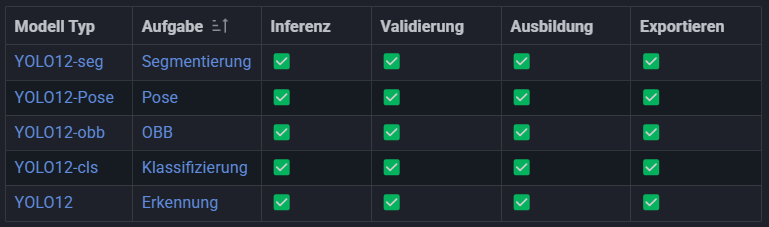
\includegraphics[width=0.85\textwidth]{data/AufgabenUndModiYOLO12.png}
    \caption{Unterstützte Aufgaben und Modis YOLOv12}
    \label{fig:YOLOv12_unterstützte_Modi}
\end{figure}